\documentclass[french, 11pt]{article}

\input{setup.tex}

\def\chapitre{7}
\def\pagetitle{Algorithmes d'approximation.}

\begin{document}

\input{title.tex}

On souhaite étudier des problèmes $\NP$-difficiles en approximant la meilleure solution.

\begin{ex}{Couverture par les sommets.}{}
    \bf{Instance:} Un graphe $G=(S,A)$.\\
    \bf{Solution:} Un sous-ensemble $S'\subset S$ tel que $\forall (s,t)\in A, ~ s\in S' \ou t\in S'$.\\
    Fonction à minimiser : $|S'|$.
    \tcblower
    \bf{Idée 1.} Tant qu'il reste des arêtes, prendre un sommet de $S$, puis retirer toutes les arêtes adjacentes.\\
    Variant de boucle : nombre d'arêtes; atteint 0. Invariant : si une arête $(s,t)$ est retirée, $s\in S'$ ou $t\in S'$.\\
    Cet algorithme n'est pas optimal.
\end{ex}

\begin{defi}{$\l$-approximation.}{}
    Pour un problème $P$ minimisant la fonction $f$, on dit d'un algorithme qu'il s'agit d'une \bf{$\l$-approximation} si pour tout instance, on a $\l f(s_{\nt{OPT}})\geq f(s_A)$ où $s_{\nt{OPT}}$ est optimale et $s_A$ la solution de l'algorithme.\\
    Dans ce cas, $f(s_A)\in[f(s_{\nt{OPT}}), \l f(s_{\nt{OPT}})]$; plus $\l$ est proche de 1, plus la solution renvoyée est optimale.\\
    On parle aussi d'approximation à facteur constant car $\l$ ne dépend pas de l'instance considérée.
    \tcblower
    Pour l'exemple précédent, on n'a pas de $\l$-approximation. Supposons qu'on en ait une, et considérons le graphe $E_k$, en étoile à $k=\lf\l\rf+1$ branches. Sur $E_k$, l'algorithme glouton peut renvoyer tous les sommets de degré 1, on a alors $f(s_{\nt{OPT}})=1$ et $f(s_A)=\lf\l\rf+1$. On aurait alors $\l\geq\lf\l\rf+1$, absurde.
\end{defi}

\begin{ex}{Modification 1.}{}
    On modifie maintenant l'algorithme pour que $s$ soit choisi comme sommet de plus haut degré.\\
    Il n'est pas optimal, par exemple sur le graphe suivant :
    \begin{center}
        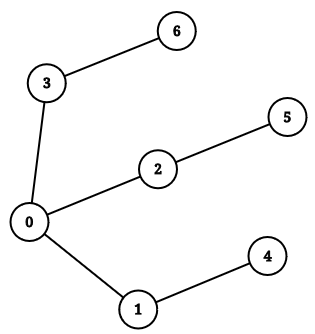
\includegraphics[scale=0.3]{graph1.png}
    \end{center}
    On n'a pas de $\l$-approximation non-plus, mais la preuve est plus complexe (exemple suivant).
\end{ex}

\pagebreak

\begin{ex}{Pas de $\l$-approximation.}{}
    On prend un graphe avec $k$ couches de sommets. La couche $i$ contient $\left\lf\frac{k}{i}\right\rf$ sommets. Chaque sommet de la couche $i$ est relié à $i$ sommets de la couche $1$. Il est le seul sommet de cette couche à être relié à ces sommets.\\
    Pour n'importe quel $k$, il existe une solution de taille $k$. Il suffit de prendre tous les sommets de la première couche. Si un sommet $s$ appartient à la couche $i>1$, son degré est exactement $i$. Les sommets de la couche 1 sont reliés à au plus $k-1$ sommets (au plus un sommet de chaque autre couche). L'algorithme glouton choisit donc le sommet de la couche $k$. Les sommets de la couche 1 sont alors de degré au plus $k-2$. Finalement, on ajoute tous les sommets n'appartenant pas à la première couche. La taille de la solution est en $\sum_{i=2}^k\left\lf\frac{k}{i}\right\rf = \Theta(k\log(k))$.\\
    S'il s'agissait d'une $\l$-approximation, on aurait $\frac{f(s_A)}{f(s_{\nt{OPT}})}\leq \l$ or $\frac{f(s_A)}{f(s_{\nt{OPT}})}\geq\sum_{i=1}^k\frac{1}{i}-2+\frac{1}{k}$.\\
    On aurait alors $\l\xrightarrow[k\to+\infty]{}+\infty$, ce qui est absurde.
\end{ex}

\vspace*{-0.5cm}

\begin{ex}{Modification 2.}{}
    On fait une dernière modification : au lieu de choisir un sommet $s$, on choisit une arête $(s,t)$ et on ajoute à la fois $s$ et $t$ dans $S'$. Ce n'est pas optimal, sur le graphe étoile, il renvoie toujours une solution de taille $2k$. Sur le graphe de l'exemple précédent aussi. Cet algorithme glouton est une $2$-approximation.
    \tcblower
    On remarque que lorsqu'on ajoute $s$ et $t$ à $S'$, on est certain qu'au moins l'un des deux appartient à la solution optimale. Ainsi, si l'algorithme glouton réalise $k$ itérations, toutes les solutions contiennent au moins $k$ sommets. L'algorithme glouton renvoie une solution à $2k$ sommets. On a $f(s_{\nt{OPT}})\geq k$, donc $2f(s_{\nt{OPT}})\geq 2k = f(s_A)$.\\
    Il s'agit bien d'une $2$-approximation.
\end{ex}

\vspace*{-0.5cm}

\begin{ex}{Programmation de tâches.}{}
    \bf{Instance.} Un nombre $p$ de processeurs, une liste de durées $(d_i)$.\\
    \bf{Solution.} Une affectation de chaque tâche à un processeur.\\
    Fonction à minimiser : temps de fin d'exécution du dernier processeur.\\
    Le problème de décision associé est $\NP$-difficile, on le montre en exhibant une réduction de $2$-Partition.
    \tcblower
    \bf{Idée 1.} Pour chaque tâche : l'affecter au processeur le moins utilisé. On peut montrer que si $p=2$, il s'agit d'une $\frac{3}{2}$-approximation, et que cette borne est atteinte. Atteint par exemple pour $(1,1,2)$.\\
    \bf{Amélioration.} On peut trier toutes les taches par durée décroissante. On obtient une $\frac{7}{6}$-approximation dans le cas à 2 processeurs. Atteint par exemple pour (3,3,2,2,2)
\end{ex}

\vspace*{-0.5cm}

\begin{prop}{Preuve d'inapproximabilité.}{}
    Le problème du Voyageur de commerce ne possède pas de $\l$-approximation en temps polynomial, sauf si $\texttt{P}=\NP$.
    \tcblower
    On raisonne par réduction comme pour la $\NP$-complétude. On suppose qu'il existe un algorithme de $\l$-approximation en temps polynomial pour le Voyageur de Commerce. On considère une instance $G=(S,A)$ de cycle hamiltonien. On cherche à construire une instance de Voyageur de Commerce sur laquelle on pourra appliquer notre $\l$-approximation. On aimerait que le résultat de celle-ci nous indique si oui ou non il y avait un cycle hamiltonien dans $G$. On veut compléter le graphe avec des arêtes de poids $f(\l)$, celles déjà présentes ayant un poids de 1. Supposons que $G$ contienne un cycle hamiltonien, la solution optimale aura un poids de $n$. Puisqu'on utilise une $\l$-approximation, on a $f(s_A)\leq \l n$. Si on prend $f(\l)=\l n$, alors si $G$ admet un cycle hamiltonien ssi $f(s_A)\leq \l n$. Si il existe un tel algorithme, on a alors un algorithme polynomial pour répondre à Cycle-Hamiltonien. Or Cycle-Hamiltonien est $\NP$-difficile, alors $\texttt{P}=\NP$.
\end{prop}

\begin{prop}{}{}
    Dans le cas où les poids respectent l'inégalité triangulaire, un algorithme d'approximation :\\
    \begin{algorithm}[H]
        \Entree{$G=(S,A)$ un graphe pondéré par $p$}
        $T$ $\gets$ arbre couvrant minimal de $G$.\\
        Enraciner cet arbre.\\
        Parcourir cet arbre en notant chaque sommet visité.\\
        Éliminer les doublons dans ce parcours pour obtenir un cycle hamiltonien.
    \end{algorithm}
    L'algorithme proposé renvoie une $2$-approximation.
    \tcblower
    On a $p(T)\leq f(s_{\nt{OPT}})$. En effet, si on prend le cycle hamiltonien et si on lui retire une arête, on obtient un arbre couvrant de poids au moins $p(T)$. Dans le parcours, chaque arête est comptée 2 fois. Le poids du chemin est donc $2p(T)$. Le chemin finalement obtenu a un poids majoré par $2f(s_{\nt{OPT}})$. Il s'agit donc bien d'une $2$-approximation. Cette borne n'est jamais atteinte, si tous les poids sont non nuls, la première inégalité est stricte : $p(T)<f(s_{\nt{OPT}})$, ce qui empêche la borne d'être atteinte.
\end{prop}

\begin{defi}{Approximation à facteur inconstant.}{}
        Planification de tâches peut être approximé à un facteur $1+\e$ en temps polynomial lorsque $p=2$.
        \tcblower
        On note $L=\max\{d_{max}, ~ \frac{1}{2}\sum_{i=1}^n d_i\}$.
        \begin{equation*}
            \frac{1}{2}\sum d_i \leq f(s_{\nt{OPT}}) \ra d_{max} \leq f(s_{\nt{OPT}}) \ra L \leq f(s_{\nt{OPT}}).
        \end{equation*}
        On partitionnera les tâches :\\
        --- Les petites de durées inférieures à $\e L$.\\
        --- Les grosses de durées supérieures à $\e L$.
\end{defi}

\begin{defi}{}{}
    --- Affecter les grosses tâches de manière optimale.\\
    --- Affecter les petites tâches de manière gloutone.
\end{defi}

\begin{prop}{Coût de l'algorithme.}{}
    Combien y-a-t-il de grosses tâches ?
    \tcblower
    Chaque grosse tâche a une durée supérieure à $\frac{\e}{2}\sum d_i$.\\
    Si on a $n$ grosse tâches, leurs poids total est d'au moins $\frac{n\e}{2}\sum d_i\leq\sum d_i$ donc $n\leq\frac{2}{\e}$.\\
    Le nombre de grosses tâches est borné par $\frac{2}{\e}$. Alors $\e$ ne dépend pas de l'instance. On peut donc le considérer comme constant.\\
    Énumérer toutes les affectations de grosses tâches n'est donc pas réalisé en temps exponentiel mais bien en temps polynomial. L'algorithme s'exécute bien en temps polynomial. Montrons qu'il s'agit bien d'une $1+\e$-approximation.\\
    --- L'affectation des petites tâches n'a pas modifié le temps d'exécution du plus lent.\\
    On considère l'instance $I^*$ restreinte avec grosses tâches. L'algorithme est optimale sur $I^*$ :
    \begin{equation*}
        f(s_{\nt{OPT}}(I)) \geq f(s_{\nt{OPT}}(I^*))
    \end{equation*}
    On a $f(s_{\nt{OPT}}(I*))=f(s_A(I))$, et $f(s_{\nt{OPT}}(I))=\geq f_{s_A(I^*)}$. Par double inégalité, $f(s_{\nt{OPT}})=f(s_A)$.\\
    --- Sinon, il existe $d_k$, une petite tâche, affectée au processeur le plus lent. Lorsqu'elle a été affectée, il s'agissait du processeur le moins occupé, son temps d'occupation était inférieur à $\frac{1}{2}\sum d_i$.\\
    Après affectation, on obtient $\frac{1}{2}\sum d_i+d_k=f(s_A)$ au plus. Alors $\frac{1}{2}\sum d_i \leq L$, $d_k\leq \e L$ puis $f(s_A)\leq (1+\e)L$.\\
    Notre algorithme s'exécute en $O(2^{\frac{1}{\e}}+P(n))$ où $P$ est un polynôme. $\e$ est en réalité un paramètre même s'il n'est pas un élément de l'instance. La complexité de l'algorithme est exponentielle en $\frac{1}{\e}$. Notre $O$ cache une constante très grande lorsque $\e$ est petit. On parle de méthode d'approximation polynomiale pour les algorithmes qui prennent en paramètre $\e$ et une instance et renvoient une $(1+\e)$-approximation en temps polynomial en la taille de l'instance. On parle de méthode d'approximation complètement polynomiale lorsque l'algorithme s'exécute aussi en temps polynomial en $\frac{1}{\e}$. 
\end{prop}

\begin{defi}{Coloration de graphe.}{}
    \bf{Instance:} Un graphe $G$.
    \bf{Solution:} Une coloration des sommets de $G$ telle que $\forall (s,t)\in A, ~ c(s) \neq c(t)$.\\
    Fonction à minimiser : Le nombre de valeurs que prend $c$.\\
    \begin{algorithm}[H]
        \Tq{il existe un sommet non coloré}{
            En choisir un $s$.\\
            Colorer $s$ avec la plus petite couleur non utilisée par ses voisins.
        }
    \end{algorithm}
    \tcblower
    Dans le cas où tous les voisins d'un sommet $s$ sont de couleur différente, on utilise $d(s)+1$ couleurs pour colorer $s$ et ses voisins. Pour colorer tout le graphe, on utilise donc au plus $d_{max}+1$ couleurs.
    Si $G$ n'est pas 2-colorable, on peut utiliser l'algorithme glouton pour avoir une $\frac{d_{max}+1}{3}$-approximation :
    \begin{equation*}
        f(s_{\nt{OPT}}) \geq 3 \ra f(s_A) \leq d_{max}+1 \ra f(s_A) = \frac{1}{3}f(s_A) \leq \frac{d_{max}+1}{3}f(s_{\nt{OPT}}).
    \end{equation*}
    S'il est 2-colorable, on trouve une coloration en temps polynomial en réalisant un parcours du graphe, au cours duquel on colorie les sommet en alternant les couleurs. Si le graphe n'est pas 2-colorable, on s'en rend compte au cours du parcours. On peut donc essayer de colorer le graphe avec deux couleurs puis d'utiliser l'algorithme glouton en cas d'échec. 
\end{defi}

\begin{defi}{3-coloration.}{}
    \begin{algorithm}[H]
        \Tq{il existe un sommet $s$ de degré supérieur à $\sqrt{n}$}{
            Colorer ses voisins avec deux nouvelles couleurs.
        }
        Colorer les sommets restants avec l'algorithme glouton.
    \end{algorithm}
    \tcblower
    À chaque itération, on colore au moins $\lceil\sqrt{n}\rceil$ sommets, on fait donc au plus $\sqrt{n}$ itérations.\\
    Le graphe des voisins de $s$ est $2$-colorable car si l'on rajoute $s$, il est 3-colorable, or, $s$ est rélié à tous les autres. Ceux-ci n'ont donc que deux couleurs possibles.\\
    À la fin de la boucle, on a utilisé $2\sqrt{n}$ couleurs au plus. L'algorithme glouton est exécuté sur un graphe de degré maximal inférieur à $\sqrt{n}$, il utilise donc au plus $\sqrt{n}+1$ couleurs.\\
    À la fin de la boucle, on a attribué $2\sqrt{n}$ couleurs au plus. L'algorithme glouton est exécuté sur un graphe de degré maximal inférieur à $\sqrt{n}$. Il utilise donc au plus $\sqrt{n+1}$ couleurs. L'algorithme colorie avec au plus $3\sqrt{n}+1$ en tout.\\
    Cette borne est rarement atteinte, car la première inégalité découle du fait d'avoir réalisé beaucoup d'itérations, tandis que la deuxième vient du fait d'en avoir fait peu.
\end{defi}



\end{document}